%05/02 - Fátima Sánchez Cabo
\part{Transcriptómica}
\chapter{RNA-Seq}
\section{Pipeline general y alineadores}
En este curso nos centraremos en los NGS de lectura corta (segunda generación). Para transcriptómica, se secuencia el cDNA generado a partir del ARNm. Este cDNA se fragmenta y se secuencia en reads cortos. Las máquinas y la forma de secuenciar es la misma que aquella vista en la asignatura "Fundamentos de Secuenciación". 

Las lecturas pueden ser solo de la primera parte del fragmento (single-reads) o lecturas pareadas para tener una mayor precisión en el alineamiento. Del secuenciador sale un fichero FastQ, el cual se alinea con un genoma de referencia en FastA. Una vez con los alineamientos, se pueden mirar las regiones con reads mapeadas que estén en el transcriptoma de referencia (GTF/GFF) y cuantificar la expresión (matriz de conteo en CSV/TSV). 

En general, el workflow es el siguiente: descargar datos, QC inicial, pre-procesamiento y QC posterior, alineamiento a una referencia, detección, conteo y análisis estadístico. En transcriptómica, se quiere cuantificar la expresión de las partes del genoma que se transcriben. Por ello, se necesita un genoma de referencia, pero también otro archivo GTF que relacione los exones con los tránscritos y los genes. El contaje por detección es el que se hace con CHIP-Seq, al secuenciar la parte del ADN genómico a la que se ha pegado un factor de transcripción predefinido. 

\begin{figure}[h]
\centering
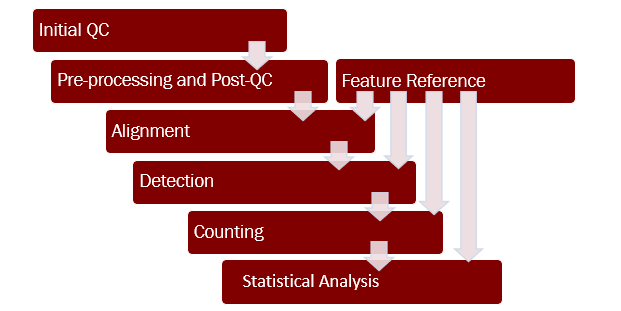
\includegraphics[width = 0.8\textwidth]{figs/ngs-analysis-workflow.png}
\end{figure}

\subsection{Control de calidad inicial}
Los objetivos del control de calidad de las lecturas crudas es detectar problemas de secuenciación, detectar adaptadores y comparar librerías para análisis posteriores. Distintos experimentos requieren interpretaciones distintas del análisis de control de calidad. Una herramienta muy utilizada para esto es FastQC. El análisis de la calidad por base, representa la distribución de las puntuaciones de calidad en todas las lecturas por la posición de cada lectura. En general, es normal que las últimas posiciones tengan una calidad algo peor que las demás, pero una buena muestra debe seguir teniendo una calidad alta. Si una muestra no tiene gran calidad, se puede optar por utilizar solo aquella porción de las muestras que tienen una calidad aceptable, pero hay que tener en cuenta que al acortar las lecturas, el mapeado puede darse en un mayor número de sitios. También se mide el contenido de cada base por posición (que debería ser bastante constante a lo largo de toda la lectura dependiendo de la "complejidad de la muestra", es decir, variedad de tránscritos diferentes) y la puntuación de calidad media por secuencia. La pipeline para el ARNm y los miRNA es la misma, pero hay peculiaridades. Los microARNs son ARNs de unos 20-30 nucleótidos que reprimen la expresión génica de los genes a los que se unen.
Dado el bajo número de miRNAs codificados por el genoma y el más reducido número expresado en cada tejido es de esperar ver perfiles de baja complejidad en las librerías de miRNAs, dádose así un patrón irregular del contenido de bases por posición.

Las secuencias sobrerrepresentadas son listas de secuencias que están presentes más veces de lo esperado por azar. La lista sobrerrepresentada se anota con el tipo de secuencia si se proporciona una lista con la que comparar. Normalmente, las secuencias adaptadoras pueden estar sobrerrepresentadas si hay altos niveles de ligaciones de dímeros de cebadores en el paso de preparación de la biblioteca. A menudo se debe a un desequilibrio entre los niveles de adaptadores y los niveles de fragmentos de muestra. Algunos RNA-Seq de tejidos particulares pueden dar también secuencias sobrerrepresentadas. Por ejemplo, las muestras de sangre contienen grandes cantidades de transcritos de hemoglobina que siempre se reportan como lecturas sobrerrepresentadas. Las muestras de miARN siempre muestran secuencias sobrerrepresentadas. Las bibliotecas de ARN total muestran secuencias sobrerrepresentadas de ARN ribosómicos.

\subsection{Preprocesado}
El preprocesado tiene como objetivo mejorar la calidad, la mapeabilidad, quitar contaminantes y sesgos, etc. Hay diferentes herramientas, como cutadapt o trim-galore. 

La calidad de las bases puede afectar al análisis de llamadas de variantes y, si es grave, también al mapeo de características. La calidad de las bases suele disminuir al final de la lectura y a veces al principio. Además, la secuenciación de baja calidad puede producir un grupo de lecturas de baja calidad a lo largo de su longitud. Es esencial eliminar las bases de baja calidad para el análisis de llamada de variantes. Para otros análisis, elimínelas sólo si afecta al rendimiento del mapeo.

\subsection{Alineamiento y mapeado}
Hay dos tipos de alineamientos: local y global. En el caso del local, se busca que en partes específicas el alineamiento sea bueno, mientras que en el global se busca meter la lectura en la secuencia completa, metiendo gaps. 

La cobertura en un segmento se mide como el número de reads que mapean a ese fragmento del genoma y la longitud de cada lectura dividido por la longitud del fragmento. Para poder hacer el mapeado se necesita la referencia en fasta, las reads en fastq y una referencia indexada. Esto es distinto de los alineadores tradicionales como BLAST. El objetivo es mapear las lecturas a las características. En transcriptómica, el alineamiento se realiza al mismo tiempo que la cuantificación. 

Lo importante es la indexación del genoma de referencia para ahorrar tiempo de computación. El genoma se corta en trozos para que sea más fácil realizar las búsquedas. Esto se puede hacer por ejemplo con BWA. 

Aunque se hable de expresión génica, los genes no se expresan, son los tránscritos. Con estas técnicas es muy complicado hilar tan fino, por lo que se cuantifican los reads al gen y contar. A la hora de alinear, si se intenta alinear reads al genoma de referencia, las reads salen del tránscrito, por lo que puede ocurrir que una parte de un read caiga en un exón y la otra parte en el otro. Esto se puede visualizar con el visor IGV. Las lecturas partidas se conocen como exon junctions. Por ello, se puede mapear al genoma permitiendo esa característica. Otra opción es alinear directamente al transcriptoma, pero es más grande que el genoma (puede haber 100.000 tránscritos definidos vs 20.000 - 30.000 genes) y puede que haya lecturas que no se puedan mapear a un tránscrito concreto. 

\begin{figure}[h]
\centering
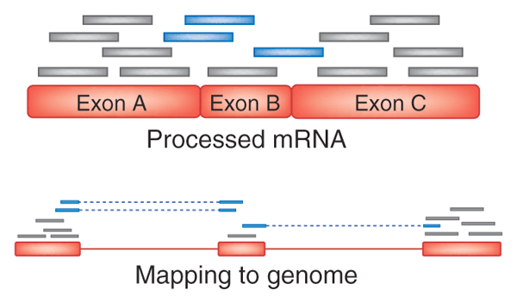
\includegraphics[width = 0.7\textwidth]{figs/Imagen1.png}
\end{figure}

\subsection{Galaxy}
Galaxy es una plataforma con muchas herramientas y workflows ya hechos para investigación biomédica intensiva en datos. Permite generar y hacer públicas pipelines. Se puede utilizar en el servidor europeo o montar un servidor local. 

Para nuestro proyecto, utilizaremos los datos del paper "Next-generation sequencing facilitates quantitative analysis of wild-type and Nrl(-/-) retinal transcriptomes". En la parte de "Related Information" se encuentran los datasets subidos a la base de datos GEO (Gene Expression Omnibus). En general, las revistas buenas exigen poner los datos en una base de datos pública. En este caso hay 6 muestras, 3 wild-type y 3 knock-out. Cada muestra en GEO tiene un ID. 

Galaxy se conecta a las bases de datos mediante API, por lo que se puede poner el link a los reads crudos y Galaxy lo lleva a nuestra sesión sin necesidad de descargarlos de las bases de datos y subirlos a Galaxy de forma manual. 

Nos vamos a descargar la información de los nombres de las muestras (los metadatos). Desde GEO, hay un acceso a SRA Run Selector donde tenemos disponibles esos datos. Hay dos tablas disponibles: metadata y lista de las accesiones con los IDs de las muestras. Los metadatos se necesita posteriormente para saber qué muestras son WT y cuáles KO, pero por ahora solo necesitamos los IDs para subir a Galaxy. El siguiente paso es decirle a Galaxy que, utilizando esos identificadores, se descarguen los FastQ. Para ello, en Get Data hay una opción de Faster Download and Extract Reads in FastQ format from NCBI SRA. Para esa herramienta se selecciona la opción de "List of SRA accessions, one per line" y se ejecuta.

Una vez con los datos, vemos que en Pair-end tenemos 0 datos y en Single-end 6, indicando que las muestras son single-end (aunque esto ya lo sabíamos porque venía en SRA Run Selector). El siguiente paso es ir a FastQC con los datos de single-end. La salida es un fichero txt con los números y un html con las imágenes.

En Ensembl nos vamos a la página de FTP Downloads donde se encuentran todas las referencias de la última versión del genoma. Para reproducir unos resultados, hay que utilizar la referencia de la fecha de publicación de los datos que se estén utilizando, pero en nuestro caso podemos utilizar la última versión generada. Como no queremos descargar el Fasta a nuestro ordenador, vamos al FastA y buscamos el fichero de primary assembly. Con click derecho, podemos copiar el enlace y en Galaxy, en Upload, se puede utilizar la función Paste/Fetch data y pegar ahí la dirección. También subimos el GTF de los cromosomas.

%\section{Expresión diferencial}
%
%\section{Análisis funcional}
%
%\chapter{CHIP-SEQ}